\section{Configuring Hardware and Software for the Dot Product Engine}
\label{sec:configDPE}

The Dot Product Engine (DPE)~\cite{hu2016dot} is a hardware accelerator for
matrix-vector multiplication using crossbar arrays to perform highly parallel
multiplications and additions through analog operations.  The concept is not
new~\cite{steinbuch1961lernmatrix,likharev2011crossnets}, with actual
implementations utilizing various technologies such as Flash, phase change
memories (PCM), and oxide-based memristors.  Circuit demonstrations have been
shown in stand alone platforms~\cite{prezioso2015training}, as well as part of
larger programmable analog computing systems~\cite{george2016programmable}.

A full architecture was recently proposed~\cite{shafiee2016isaac} that
integrates analog DPE components in a scalable, pipelined flow with digital
routing, buffers, and other components to flexibly support inference
computations for a broad range of Convolutional Neural Networks (CNN).  An
ISAAC chip is contains a number of tiles, composed of eDRAM buffers to store
input values, a number of in-situ multiply-accumulate (IMA) units, and output
registers to aggregate results.  All components are connected with a shared
bus.  Each IMA contains several crossbar arrays as well as shared ADCs.

A key performance aspect of the ISAAC architecture is the use of in-memory
processing, that is, memristor arrays not only store neural network weights,
but are also the location for computation. This reduction in data-fetching is
fundamental for performance improvement, but also imposes a strict data flow
that needs to be pipelined. Additionally, tiles can be partitioned between
different CNNs for a specific task.

Another parameter that impacts performance is the bit precision in matrix-vector
multiplication operations. Neural networks are highly tolerant of low
precision~\cite{courbariaux2014low, rastegari2016xnor, zhou2016dorefa}, which
reduces the load on ADCs. The precision needed to implement each neural network
layer is an important parameter to trade-off performance versus classification
accuracy.  Choosing the optimal operating point requires careful management.

Mapping neural network layers of various sizes to the appropriate physical
memristor crossbar arrays is a complex task.   Simply placing the neural
network layer in the largest possible array can lead to larger errors and
slower operating speeds.

The configuration optimization of data flow pipelines, tile partitioning,
operation bit precision and neural network mapping present opportunities to use
autotuners in the exploration of DPE hardware and software design spaces.  This
section presents our ongoing efforts on elaborating a search space for
autotuning that represents the hardware design space of the DPE.  We are
working with Hewlett-Packard Enterprise on this project.

\subsection{Background}

Many special-purpose accelerators have been proposed for neural network
acceleration~\cite{chen2014dadiannao,chi2016prime,shafiee2016isaac}, for which
dot-products are a fundamental operation.  Memristor-based DPEs have been shown
to be particularly promising~\cite{shafiee2016isaac} for computation patterns,
such as inference, where one of the operands is constant and frequently reused.
The DPE accelerates this operation by programming the constant operand into a
memristor crossbar and performing the computation in-situ with a streaming
input.

\subsection{Autotuning the Dot Product Engine}

Figure~\ref{fig:dpe-stack} shows the steps needed to generate a DPE
implementation from a hardware configuration or specification and to generate
application code using software parameters. These two steps present
autotuning opportunities for hardware and software parameters.

\begin{figure}[htpb]
    \centering
    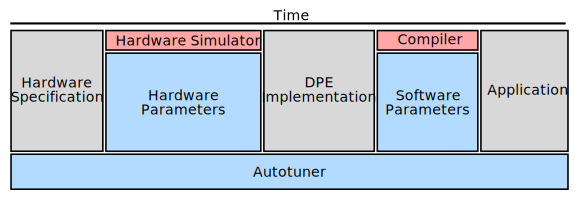
\includegraphics[width=.65\textwidth]{./images/dpe-stack}
    \caption{Steps from DPE hardware to software design and implementation}
    \label{fig:dpe-stack}
\end{figure}

We are using cycle-accurate simulators to obtain hardware metrics for different
DPE configurations, since the DPE architecture is still not defined.  The time
to obtain a working architecture simulation for a set of hardware parameters is
fast, since it consists of loading a configuration file.  We expect to use
simulators to explore the hardware design space before producing a prototype,
and autotuning will aid this exploration for different applications.
Figure~\ref{fig:overview-dpe-hard} shows the autotuner representation and time
scale for the current simulator-based workflow.

\begin{figure}[htpb]
    \centering
    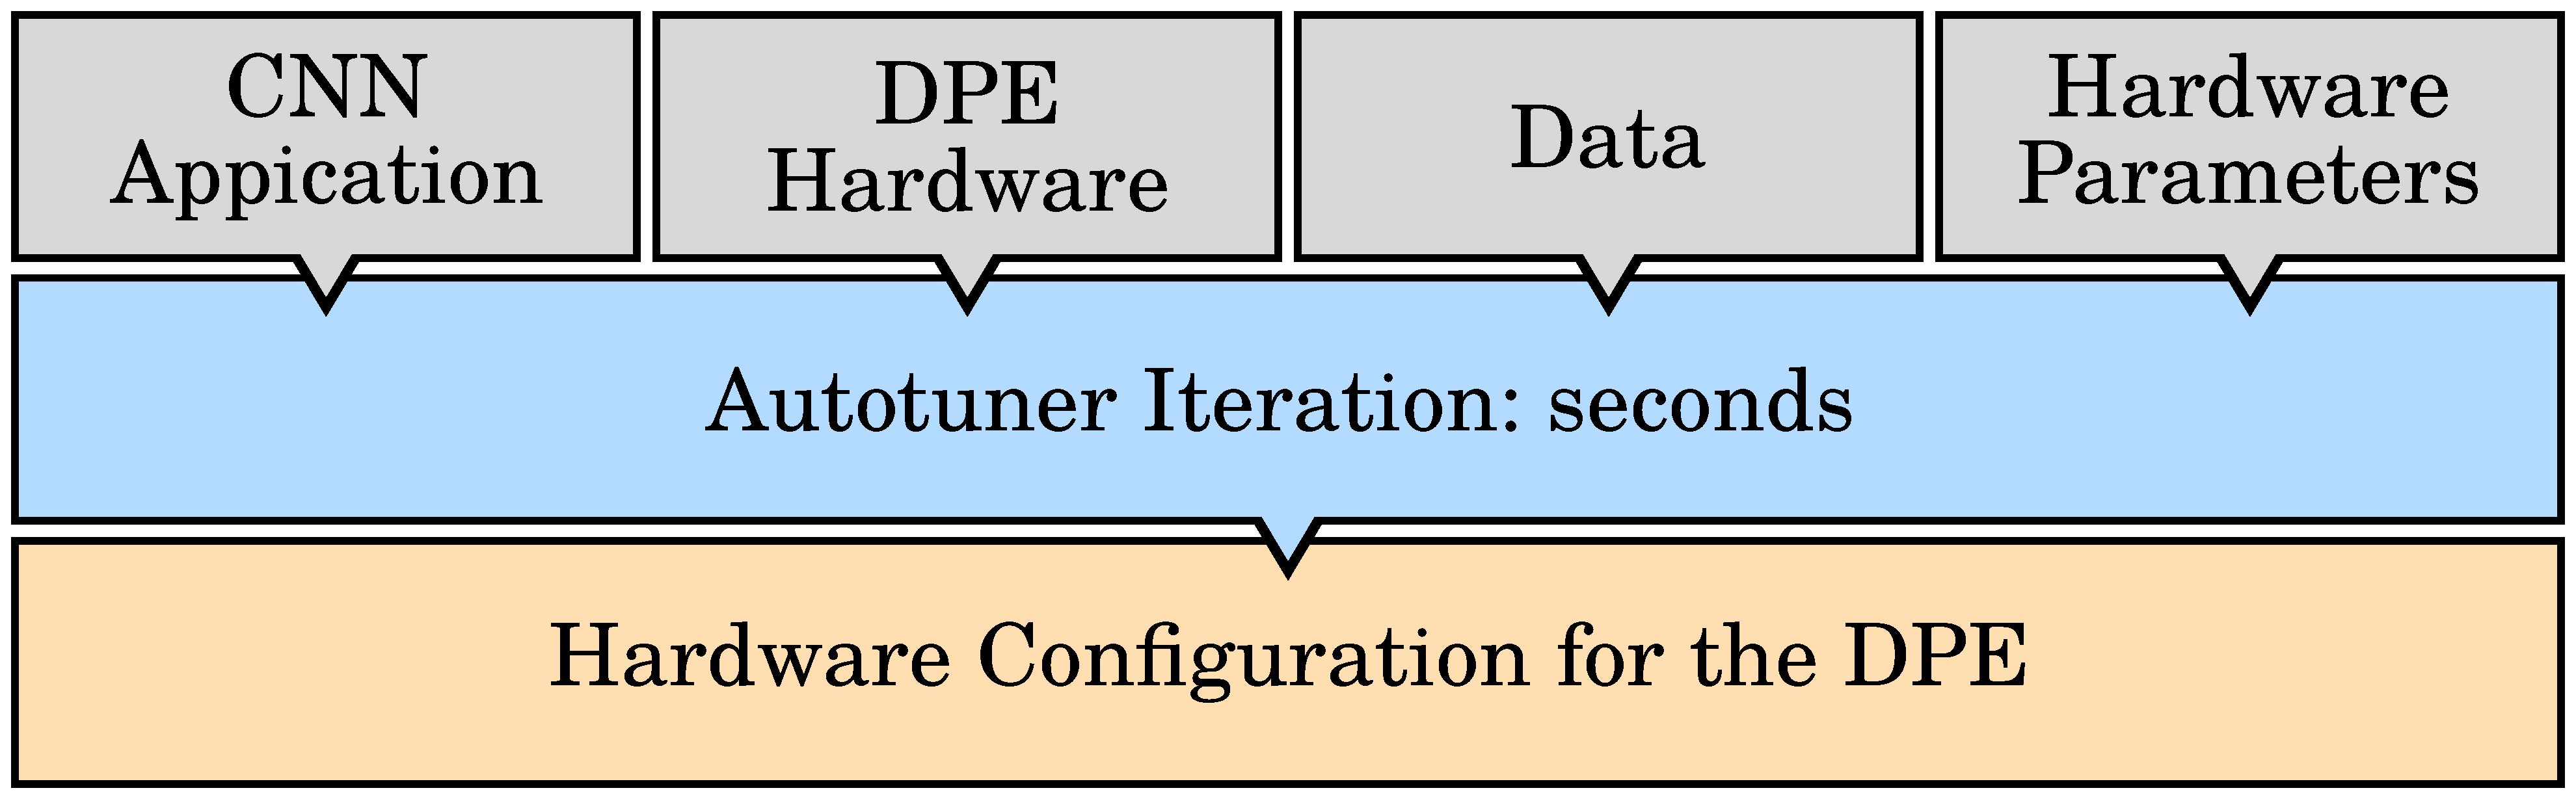
\includegraphics[width=.65\textwidth]{./images/overview_dpe_hard}
    \caption{Autotuner representation and time scale for hardware parameter
    autotuning}
    \label{fig:overview-dpe-hard}
\end{figure}

Figure~\ref{fig:overview-dpe-app} shows the autotuner representation and time
scale for software parameter autotuning. The simple applications that we are
using now have no parameters and take time in the order of seconds to complete.
The DPE code for these applications is also written by hand. We expect that the
code for future applications will be generated by a compiler, and compiling and
running time may vary.

\begin{figure}[htpb]
    \centering
    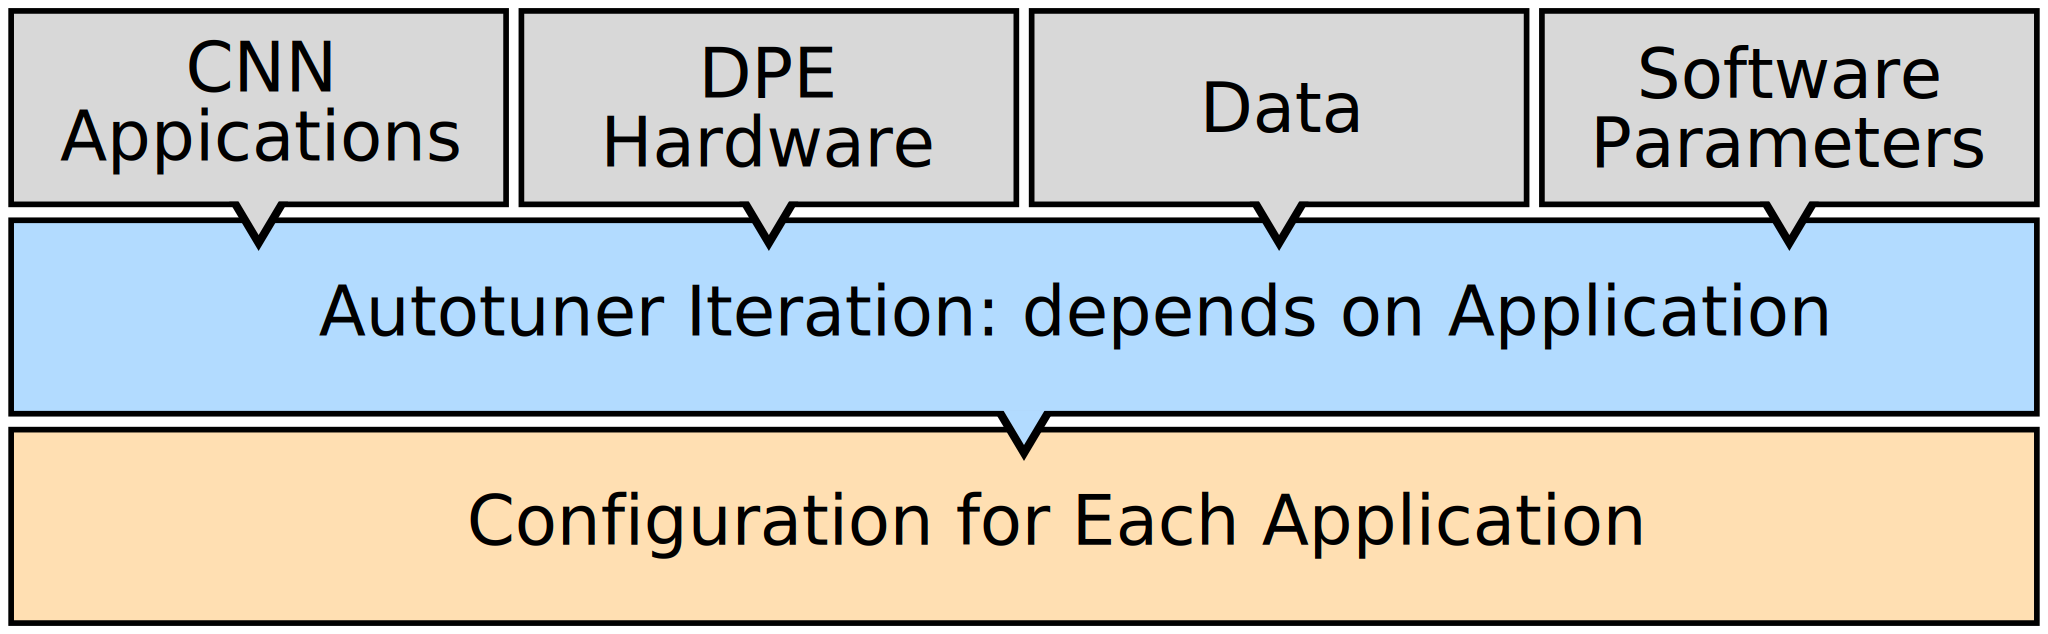
\includegraphics[width=.65\textwidth]{./images/overview_dpe_app}
    \caption{Autotuner representation and time scale for software parameter
    autotuning}
    \label{fig:overview-dpe-app}
\end{figure}

\subsection{Autotuner \& Search Space}
\label{sec:DPEautotuning}

This section presents the autotuner that we are implementing and the
preliminary search space we developed with DPE hardware design parameters.

\subsubsection{Autotuner}

We are implementing an autotuner for DPE hardware parameters.  We did not
consider software parameters in this stage, since we are only targeting simple
applications initially. The autotuner is being implemented using the autotuning
library we are developing in the Julia language. The source code for the
autotuner is available at GitHub~\footnote{Hosted at
\url{https://github.com/phrb/dpe-emulate-autotuner}}The library is described in
detail in chapter~\ref{chap:julia}.

We did not want the autotuner's performance to impose limits to the size of the
hardware design space that could be explored for the DPE. Using Julia's
parallel and distributed programming interfaces, our library supports execution
in many-core machines and distributed environments. Future experiments will
partition the hardware design space between multiple instances of parallel
search techniques, and target hardware metrics of tiles, IMAs and DACs/ADCs.

\subsubsection{Search Space}

Table \ref{tab:hard-soft-params} shows hardware and software parameters that
define a design and reconfiguration space for the DPE. The impact of these
parameters on several metrics can be measured using analytical models and
simulations.  Table \ref{tab:metrics-measurements} shows metrics and
measurement strategies that can be optimized for the DPE.

\begin{table}[htpb]
\centering
\begin{tabular}{@{}p{0.45\columnwidth}p{0.45\columnwidth}@{}}
\toprule
\textbf{Hardware} & \textbf{Software} \\ \midrule
Routing tables, eDRAM buffer size; bit size in IMA, layer; bus width; crossbar \& IMA number in tiles & Memristor arrays, layers \& routing tables mapping  \\
\addlinespace
ADC hardware configuration and heterogeneous tile designs & ADC and tile usage \\ \bottomrule
\addlinespace
\end{tabular}
\caption{Tunable software and hardware DPE parameters
}
\label{tab:hard-soft-params}
\end{table}

\begin{table}[htpb]
\centering
\begin{tabular}{@{}p{0.46\columnwidth}p{0.46\columnwidth}@{}}
\toprule
\textbf{Metrics} & \textbf{Measurements} \\ \midrule
Bandwidth, latency, execution time, router area, throughput & Modelled area and power overhead for components \\
\addlinespace
Computation, power, crossbar efficiency & Cycle accurate simulation for: tile communication; eDRAM access \\
\addlinespace
Usability, flexibility & Empirical, qualitative \\ \bottomrule
\addlinespace
\end{tabular}
\caption{Tuning metrics \& measurement strategies for DPE}
\label{tab:metrics-measurements}
\end{table}

\todo[inline,author=Pedro,color=cyan]{Add results if possible}

\subsection{Summary}
\label{subsec:DPEconcl}

This work is still ongoing. The capability of changing each hardware metric
still being studied and implementing, and code for the DPE simulator is still
written by hand. We expect to advance more in the next months, leveraging code
generators and simulator improvements that the HPE work group produces to
explore the hardware and software design spaces with autotuning.
